\chapter{Mesura de la resistència d'un metall}
\begin{resum}
	L'objectiu d'aquesta pràctica és la mesura experimental de la resistivitat d'un metall. Més concretament, s'ha centrat en la dependència de la resistivitat amb la temperatura. La teoria indica que la resistivitat d'un material, i, en conseqüència, la seva resistència, augmenten linealment amb la temperatura. El nostre experiment, realitzat en un rang de temperatures comprès entre els $\SI{-150}{\celsius}$ i els $\SI{265}{\celsius}$ corrobora aquesta aquesta predicció, ja que la regressió lineal realitzada a partir de les dades de la resistència del metall enfront la temperatura té un coeficient de correlació de $0.997$. S'ha calculat també el factor de proporcionalitat entre la resistència i la temperatura, amb un valor de $\data{0.359}{0.003}{\ohm.\celsius^{-1}}$, i l'ordenada a l'origen, de valor $\data{106.9}{0.4}{\ohm}$.
\end{resum}

\section{Introducció}
En nombrosos conductors, existeix una relació entre el camp elèctric $\vec{E}$ i la densitat de corrent $\vec{J}$ coneguda com la llei d'Ohm, de manera que $\vec{J}=\rho\vec{E}$, on $\rho$ denota la resistivitat del material.

Com que la resistència d'un material de longitud $L$ i secció constant $A$ es pot escriure com $R=\frac{\rho L}{A}$ i la resistivitat augmenta linealment amb la temperatura \( \theta \), en primera aproximació, podem considerar que la resistència d'un material vindrà donada per 
\begin{equation} \label{eq:regressio}
R(\theta)=R_0(1+\beta\theta)
\end{equation}

El nostre objectiu és demostar experimentalment aquesta relació per un material concret i trobar-ne els valors numèrics dels paràmetres $R_0$ i $\beta$.

\section{Mètode experimental}
L'experiment requereix de la mesura de la temperatura del metall i de la seva resistència en diferents moments.

Per tal de mesurar la temperatura es disposa de dos termòmetres de mercuri amb precisió de \SI{1}{\celsius}. Un dels dos s'usa en el rang de temperatures altes ---fins a uns $\SI{300}{\celsius}$--- i l'altre, en el rang de temperatures baixes ---fins a uns $ \SI{-200}{\celsius}$---.

Per tal de mesurar la resistència del material s'ha usat una variació del pont de Wheatstone ---\ref{fig:wheatstone}---, el pont de fil. Com es pot apreciar, el circuit consisteix en quatre resistències connectades en forma de paral·lelogram, tres d'elles conegudes i una desconeguda. Els vèrtex del paral·lelogram s'uneixen amb un amperímetre per tal de mesurar la intensitat que hi circula. El pont estarà equilibrat quan l'amperímetre marqui zero, i llavors podrem trobar la resistència desconeguda a partir de
\begin{equation*}
\frac{R_1}{R_2}=\frac{R_3}{R_4}.
\end{equation*}

\begin{figure}[htb]
	\centering
	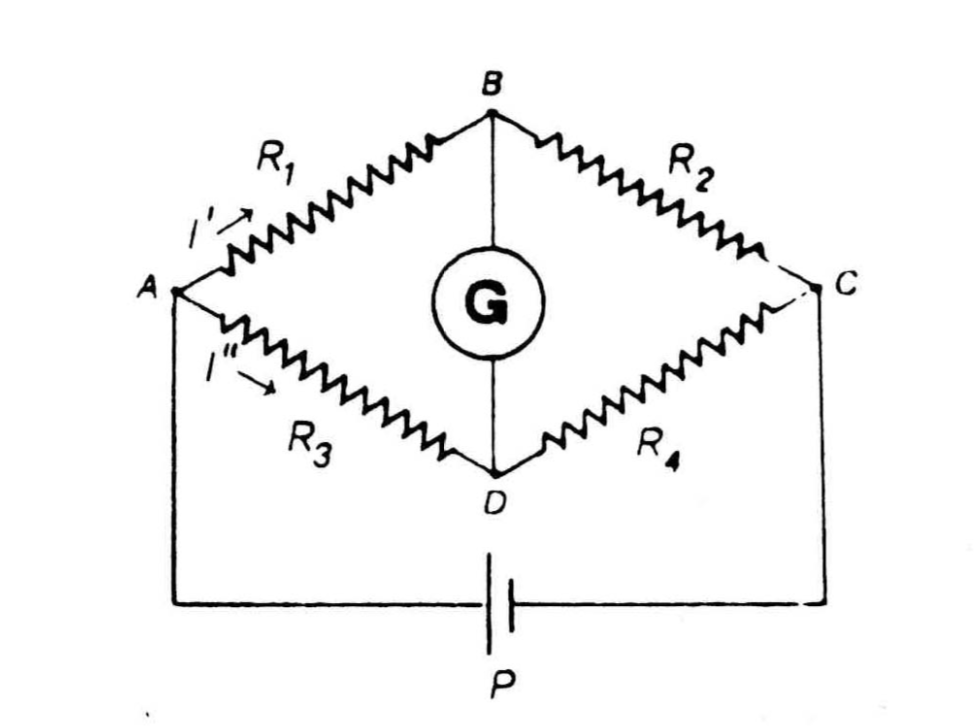
\includegraphics[scale=0.4]{pont.png}
	\caption{Esquema del pont de Wheatstone}
	\label{fig:wheatstone}
\end{figure}

\begin{figure}[htb]
	\centering
	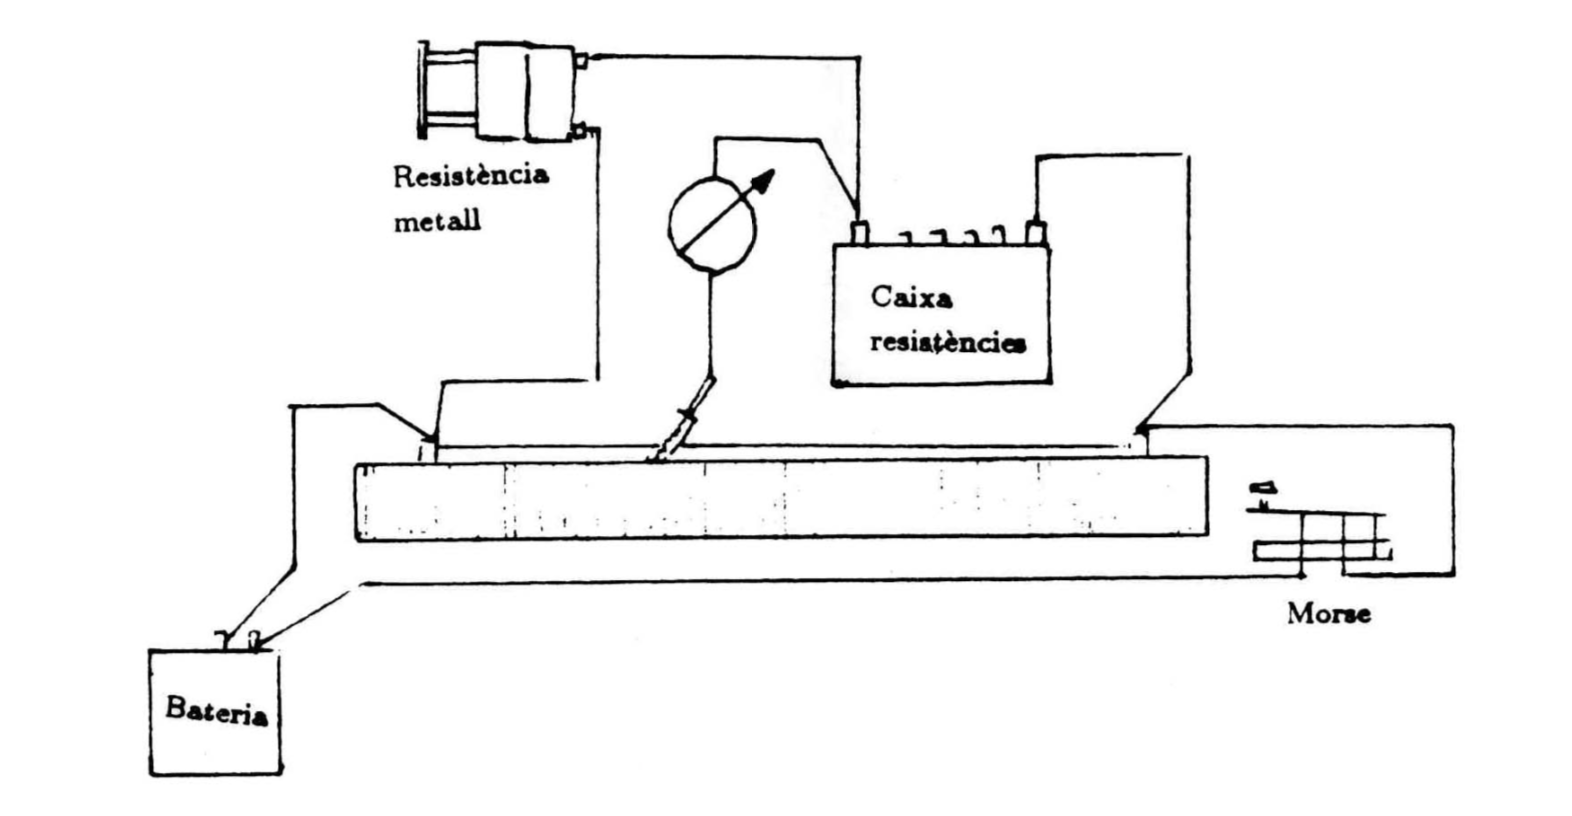
\includegraphics[scale=0.4]{muntatge.png}
	\caption{Esquema del muntatge experimental}
	\label{fig:muntatge resistencia}
\end{figure}

En el pont de fil, dues de les resistències se substitueixen per un fil de longitud coneguda i un cursor que es pot moure per sobre. D'aquesta manera, existeix una relació directa entre el quocient de les longituds i el quocient de les seves resistències. Usant una tercera resistència coneguda, $R_2$, la resistència incògnita, $R_1$, ve donada, quan el pont està equilibrat, per
\begin{equation}\label{eq: <pont>}
R_1=\frac{x}{L-x}R_2
\end{equation}
on $x$ denota la longitud de fil a l'esquerra del cursor i $L$ la longitud total del fil. El muntatge experimental es pot veure a la \cref{fig:muntatge resistencia}. 

Per poder mesurar en el rang d'altes temperatures s'ha escalfat la resistència en un forn. S'ha deixat que la seva temperatura pugés fins a uns $\SI{300}{\celsius}$ i s'han pres les mesures mentre es refredava. Per pendre les mesures en el rang de baixes temperatures, la resistència s'ha submergit en un bany de nitrogen líquid. Un cop extreta del bany, la resistència s'ha mantingut en les proximitats del nitrogen per ralentir-ne el procés d'escalfament i així poder prendre les mesures amb més precisió. 

\section{Resultats}
La \cref{tab:temp i resistencia} mostra la longitud $x$ a l'esquerra del fil a cada temperatura determinada, juntament amb la resistència del metall, usant \ref{eq: <pont>}. La longitud total del fil ha estat fixada en $L=\data{1.000}{0.001}{\meter}$ i la resistència externa en $R_1=\data{100}{1}{\ohm}$.

La regressió lineal amb les dades de la \cref{tab:temp i resistencia} es mostra a la figura \ref{fig:temp v resistencia}. El coeficient de correlació obtingut és de 0.997, el que demostra la linealitat de les dades en l'experiment considerat. S'han obtingut valors de $\data{0.359}{0.003}{\ohm\per\celsius}$ pel pendent i de $\data{106.9}{0.4}{\ohm}$ per l'ordenada a l'origen. Relacionant aquests valors amb l'\cref{eq:regressio} s'obté $R_0=\data{106.9}{0.4}{\ohm}$ i $\beta=\data{336}{3e-5}{\ohm\per\celsius}$.

\begin{figure} [htb]
	\centering
	\small \sffamily
	% % GNUPLOT: LaTeX picture with Postscript
\begingroup
\sffamily \small
  \makeatletter
  \providecommand\color[2][]{%
    \GenericError{(gnuplot) \space\space\space\@spaces}{%
      Package color not loaded in conjunction with
      terminal option `colourtext'%
    }{See the gnuplot documentation for explanation.%
    }{Either use 'blacktext' in gnuplot or load the package
      color.sty in LaTeX.}%
    \renewcommand\color[2][]{}%
  }%
  \providecommand\includegraphics[2][]{%
    \GenericError{(gnuplot) \space\space\space\@spaces}{%
      Package graphicx or graphics not loaded%
    }{See the gnuplot documentation for explanation.%
    }{The gnuplot epslatex terminal needs graphicx.sty or graphics.sty.}%
    \renewcommand\includegraphics[2][]{}%
  }%
  \providecommand\rotatebox[2]{#2}%
  \@ifundefined{ifGPcolor}{%
    \newif\ifGPcolor
    \GPcolortrue
  }{}%
  \@ifundefined{ifGPblacktext}{%
    \newif\ifGPblacktext
    \GPblacktextfalse
  }{}%
  % define a \g@addto@macro without @ in the name:
  \let\gplgaddtomacro\g@addto@macro
  % define empty templates for all commands taking text:
  \gdef\gplbacktext{}%
  \gdef\gplfronttext{}%
  \makeatother
  \ifGPblacktext
    % no textcolor at all
    \def\colorrgb#1{}%
    \def\colorgray#1{}%
  \else
    % gray or color?
    \ifGPcolor
      \def\colorrgb#1{\color[rgb]{#1}}%
      \def\colorgray#1{\color[gray]{#1}}%
      \expandafter\def\csname LTw\endcsname{\color{white}}%
      \expandafter\def\csname LTb\endcsname{\color{black}}%
      \expandafter\def\csname LTa\endcsname{\color{black}}%
      \expandafter\def\csname LT0\endcsname{\color[rgb]{1,0,0}}%
      \expandafter\def\csname LT1\endcsname{\color[rgb]{0,1,0}}%
      \expandafter\def\csname LT2\endcsname{\color[rgb]{0,0,1}}%
      \expandafter\def\csname LT3\endcsname{\color[rgb]{1,0,1}}%
      \expandafter\def\csname LT4\endcsname{\color[rgb]{0,1,1}}%
      \expandafter\def\csname LT5\endcsname{\color[rgb]{1,1,0}}%
      \expandafter\def\csname LT6\endcsname{\color[rgb]{0,0,0}}%
      \expandafter\def\csname LT7\endcsname{\color[rgb]{1,0.3,0}}%
      \expandafter\def\csname LT8\endcsname{\color[rgb]{0.5,0.5,0.5}}%
    \else
      % gray
      \def\colorrgb#1{\color{black}}%
      \def\colorgray#1{\color[gray]{#1}}%
      \expandafter\def\csname LTw\endcsname{\color{white}}%
      \expandafter\def\csname LTb\endcsname{\color{black}}%
      \expandafter\def\csname LTa\endcsname{\color{black}}%
      \expandafter\def\csname LT0\endcsname{\color{black}}%
      \expandafter\def\csname LT1\endcsname{\color{black}}%
      \expandafter\def\csname LT2\endcsname{\color{black}}%
      \expandafter\def\csname LT3\endcsname{\color{black}}%
      \expandafter\def\csname LT4\endcsname{\color{black}}%
      \expandafter\def\csname LT5\endcsname{\color{black}}%
      \expandafter\def\csname LT6\endcsname{\color{black}}%
      \expandafter\def\csname LT7\endcsname{\color{black}}%
      \expandafter\def\csname LT8\endcsname{\color{black}}%
    \fi
  \fi
    \setlength{\unitlength}{0.0500bp}%
    \ifx\gptboxheight\undefined%
      \newlength{\gptboxheight}%
      \newlength{\gptboxwidth}%
      \newsavebox{\gptboxtext}%
    \fi%
    \setlength{\fboxrule}{0.5pt}%
    \setlength{\fboxsep}{1pt}%
\begin{picture}(5668.00,3400.00)%
    \gplgaddtomacro\gplbacktext{%
      \csname LTb\endcsname%%
      \put(1078,704){\makebox(0,0)[r]{\strut{}\num{0}}}%
      \put(1078,1117){\makebox(0,0)[r]{\strut{}\num{0.05}}}%
      \put(1078,1529){\makebox(0,0)[r]{\strut{}\num{0.1}}}%
      \put(1078,1942){\makebox(0,0)[r]{\strut{}\num{0.15}}}%
      \put(1078,2354){\makebox(0,0)[r]{\strut{}\num{0.2}}}%
      \put(1078,2767){\makebox(0,0)[r]{\strut{}\num{0.25}}}%
      \put(1078,3179){\makebox(0,0)[r]{\strut{}\num{0.3}}}%
      \put(1210,484){\makebox(0,0){\strut{}\num{5}}}%
      \put(1790,484){\makebox(0,0){\strut{}\num{10}}}%
      \put(2370,484){\makebox(0,0){\strut{}\num{15}}}%
      \put(2950,484){\makebox(0,0){\strut{}\num{20}}}%
      \put(3531,484){\makebox(0,0){\strut{}\num{25}}}%
      \put(4111,484){\makebox(0,0){\strut{}\num{30}}}%
      \put(4691,484){\makebox(0,0){\strut{}\num{35}}}%
      \put(5271,484){\makebox(0,0){\strut{}\num{40}}}%
      \put(4111,1529){\makebox(0,0){\strut{}$r^2$ = \num{0.999}}}%
    }%
    \gplgaddtomacro\gplfronttext{%
      \csname LTb\endcsname%%
      \put(198,1941){\rotatebox{-270}{\makebox(0,0){\strut{}$\mathsf{F \ (\si{mN})}$}}}%
      \put(3240,154){\makebox(0,0){\strut{}$\mathsf{I^2 \ (\si{A})}$}}%
    }%
    \gplbacktext
    \put(0,0){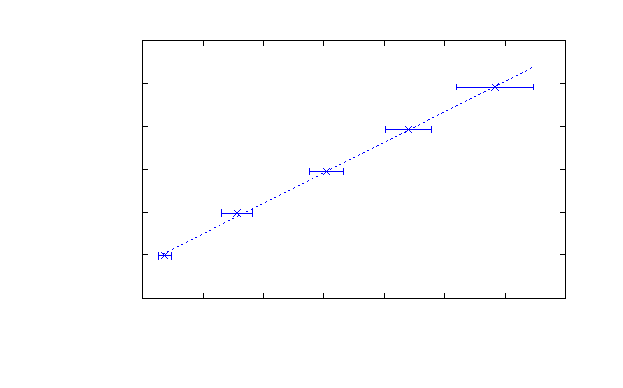
\includegraphics{forca-intensitat}}%
    \gplfronttext
  \end{picture}%
\endgroup

	\caption{Resistència en funció de la temperatura}
	\label{fig:temp v resistencia}
\end{figure}

\section{Conclusions}
S'ha comprovat experimentalment la relació lineal entre la temperatura del metall usat i la seva resistència. El coeficient de correlació, de 0.997, demostra que existeix una relació com la descrita en l'\ref{eq:regressio}. A més, s'han pogut determinar els paràmetres $\beta$ i $R_0$, amb valors de $\data{336}{3e-5}{\per\celsius}$ i $\data{106.9}{0.4}{\ohm}$ respectivament.








\begin{table}[p] 
	\centering \footnotesize \sffamily
	\caption{Mesures experimentals de la resistència a diferents temperatures. El voltatge subministrat és de \data{3.1}{0.2}{V}}
	\label{tab:temp i resistencia}
	\begin{tabular}{SSS}
		\toprule
		{Temperatura (\data{}{1}{\celsius}) } & {Longitud \( x \) (\data{}{0.001}{m})} & {Resistència (\si{\ohm})} \\
		\midrule
		265 & 0.664 & 198 \pm 9 \\
		260 & 0.668 & 201 \pm 9 \\
		255 & 0.665 & 199 \pm 9 \\
		250 & 0.664 & 198 \pm 9 \\
		245 & 0.663 & 197 \pm 9 \\
		240 & 0.661 & 195 \pm 9 \\
		235 & 0.659 & 193 \pm 9 \\
		230 & 0.657 & 192 \pm 9 \\
		225 & 0.655 & 190 \pm 9 \\
		220 & 0.654 & 189 \pm 9 \\
		210 & 0.646 & 182 \pm 8 \\
		200 & 0.643 & 180 \pm 8 \\
		190 & 0.637 & 175 \pm 8 \\
		180 & 0.630 & 170 \pm 8 \\
		170 & 0.627 & 168 \pm 7 \\
		160 & 0.622 & 165 \pm 7 \\
		155 & 0.620 & 163 \pm 7 \\
		150 & 0.616 & 160 \pm 7 \\
		145 & 0.613 & 158 \pm 7 \\
		140 & 0.610 & 156 \pm 7 \\
		135 & 0.608 & 155 \pm 7 \\
		130 & 0.605 & 153 \pm 7 \\
		125 & 0.603 & 152 \pm 7 \\
		120 & 0.600 & 150 \pm 6 \\
		115 & 0.597 & 148 \pm 6 \\
		110 & 0.593 & 146 \pm 6 \\
		105 & 0.585 & 141 \pm 6 \\
		23 & 0.520 & 108 \pm 5 \\
		-20 & 0.485 & 94 \pm 4{}\\
		-25 & 0.484 & 94 \pm 4 \\
		-30 & 0.481 & 93 \pm 4 \\
		-35 & 0.478 & 92 \pm 4 \\
		-40 & 0.474 & 90 \pm 4 \\
		-45 & 0.470 & 88 \pm 4 \\
		-49 & 0.468 & 88 \pm 4 \\
		-55 & 0.464 & 87 \pm 4 \\
		-60 & 0.459 & 85 \pm 4 \\
		-65 & 0.457 & 84 \pm 4 \\
		-70 & 0.452 & 82 \pm 3 \\
		-75 & 0.447 & 81 \pm 3 \\
		-80 & 0.445 & 80 \pm 3 \\
		-85 & 0.441 & 79 \pm 3 \\
		-90 & 0.436 & 77 \pm 3 \\
		-95 & 0.431 & 76 \pm 3 \\
		-100 & 0.424 & 74 \pm 3 \\
		-105 & 0.417 & 72 \pm 3 \\
		-110 & 0.409 & 69 \pm 3 \\
		-115 & 0.398 & 66 \pm 3 \\
		-150 & 0.365 & 57 \pm 3 \\
		\bottomrule
	\end{tabular}
\end{table}  
